\newif\ifglobal

%%%%%%%%%%%%%%%%%%%%%%%
%%% Compile to view %%%
%%%%%%%%%%%%%%%%%%%%%%%

%%%%%%%%%%%%%%%%%%%%%%%%%%%%%%%%%%%%%%%%%%%%%%%%%%%
%%% Readme:                                     %%%
%%% https://www.overleaf.com/read/bwdjvfjksvjy/ %%%
%%%%%%%%%%%%%%%%%%%%%%%%%%%%%%%%%%%%%%%%%%%%%%%%%%%

% >>> M?: marks a module setting number or important notice

% >>> M4: Set {./relative-path} to external files for this module <<<
\def \modulefiles {./13-BOOTCTRL}
% To add an external file, use:
% (Replace '---' with actual filename)
% '\input{\modulefiles/tables/---.tex}' for tables
% '\includegraphics{\modulefiles/figures/---}' for figures
% '\subfile{\modulefiles/---}' for register files

% >>> M1: This module is in global project? <<<
% 'YES' - uncomment; 'NO' - comment out
\globaltrue

\ifglobal
    \documentclass[main\_\_CN.tex]{subfiles}

\else
    % Font "FandolSong-Regular" used by ctex does not have GSUB table.
    % It causes warnings that do not affect compilation and can be ignored.
    \PassOptionsToPackage{quiet}{fontspec}

    \documentclass[openany, 10pt]{book}

    % >>> M2: In ./chip-spec-settings/preamble-trm-module, also find
    %         settings for visibility of todo notes, watermark <<<
    \usepackage{preamble-trm-module}


    % Enable Chinese typesetting
    \usepackage{ctex}

    % >>> M3: Temporary labels in Chinese
    %         you can add your own labels there <<<
    \myexternaldocument{temp-labels-cn}

\fi %\ifglobal


\setcounter{secnumdepth}{4}


% >>> M5: If this module needs any updates in
% './chip-spec-settings/preamble-trm-module.sty'
% (include additional package, etc.), contact your module PM
% or create the file './chip-spec-settings/changelog.tex' make the
% necessary updates yourself and document them in this file <<<

\raggedright


\begin{document}


% Sets language into which pre-defined bits of text are translated
\selectlanguage{chinese}

% Do not delete this block
\ifglobal
% Add the following front matter if
% this module is outside of global project
\else
    \InputIfFileExists{readme}{}{}
    {\let\clearpage\relax \listoftodos}
    {\let\clearpage\relax \listofdonetodos}
    \tableofcontents
    %\listoftables
    %\listoffigures
\fi


%%%%%%%%%%%%%%%%%%%%%%%%%
%%% TRM Module Begins %%%
%%%%%%%%%%%%%%%%%%%%%%%%%

\hypertarget{bootctrl}{}
\chapter{芯片 Boot 控制}
\label{mod:bootctrl}
\section{概述}

芯片 Boot 过程以及芯片的某些功能是在上电或硬件复位时由 Strapping 管脚和一些 eFuse 比特位来确定的，具体包括以下功能：

\begin{itemize}
    \item 控制 Boot 模式
    \item 控制 ROM 代码日志打印
    \item 控制 JTAG 信号源
\end{itemize}

\chipname{} 共有五个 Strapping 管脚：
\begin{itemize}
    \item GPIO34
    \item GPIO35
    \item GPIO36
    \item GPIO37
    \item GPIO38
\end{itemize}

在芯片复位过程中（请参考章节 \ref{mod:resclk} \textit{\nameref{mod:resclk}}），硬件将采样 Strapping 管脚电平存储到锁存器中，并一直保持到芯片掉电。Strapping 管脚的锁存值可以通过软件从寄存器 \hyperref[fielddesc:GPIOSTRAPPING]{GPIO\_STRAPPING}
中读取。

\section{功能描述}
本小节主要介绍芯片复位时的功能以及控制该功能使用到的 Strapping 管脚和 eFuse 组合模式。

\begin{importantlisting}\\
请使用本章节所介绍的组合，其它组合可能会导致不可控结果。
\end{importantlisting}

\subsection{默认配置}

GPIO35 默认连接内部上拉电阻。如果这一管脚没有外部连接或者连接的外部线路处于高阻抗状态，内部弱上拉将决定这一管脚输入电平的默认值，如表 \ref{tab:bootctrl-default-config-strapping-pins} 所示。

\newpage
\begin{longtable}[c]{|p{1.5cm}|c|}
\caption{管脚默认上拉/下拉}
\label{tab:bootctrl-default-config-strapping-pins} \\
    \hline
    \rowcolor{lightgray}
  \textbf{管脚} & \textbf{默认值} \\ \hline
  \textbf{GPIO34} & 浮空 \\ \hline
  \textbf{GPIO35} & 上拉 \\ \hline
  \textbf{GPIO36} & 浮空 \\ \hline
  \textbf{GPIO37} & 浮空  \\ \hline
  \textbf{GPIO38} & 浮空 \\ \hline
\end{longtable}

如需改变 Strapping 管脚的默认值，用户可以应用外部下拉/上拉电阻，或者应用主机 MCU 的 GPIO 来控制 \chipname{} 上电复位时的 Strapping 管脚电平。复位释放后，Strapping 管脚和普通管脚功能相同。

\subsection{Boot 模式控制}

复位释放后，GPIO35，GPIO36，GPIO37 和 GPIO38 共同控制 Boot 模式。表 \ref{tab:bootctrl-boot-mode-control} 列出了 GPIO35，GPIO36，GPIO37 和 GPIO38 的 Strapping 值及其对应的系统 Boot 模式。


\begin{ThreePartTable}

\begin{TableNotes}
    \item[1] x：任何取值均不会对结果有影响，因此可忽略。
    \item[2] Joint Download 模式：Joint Download 模式下支持以下下载方式：
    \begin{itemize}
        \item USB-Serial-JTAG Download
        \item UART Download
        \item SPI Slave Download
        \item USB 2.0 OTG Download

    \end{itemize}
    \item[3] SPI Download 模式：只有使用 SPI Download 模式时才需要预留 GPIO37 和 GPIO38。GPIO37 和 GPIO38 默认浮空，在复位时处于高阻抗状态。
    \item[4] 无效组合：该组合会触发意外行为，应当避免。

\end{TableNotes}
\begin{longtable}[c]{|p{3.5cm}|c|c|c|c|c|}
\caption{系统 Boot 模式}
\label{tab:bootctrl-boot-mode-control} \\
    \hline
    \rowcolor{lightgray}
  \textbf{ Boot 模式} & \textbf{GPIO35} & \textbf{GPIO36} & \textbf{GPIO37} & \textbf{GPIO38}\\
    \hline
    \endfirsthead
    \insertTableNotes
    \endlastfoot
  SPI Boot 模式（默认） & 1 & x\tnote{1} & x & x \\ \hline
  Joint Download 模式\tnote{2} & 0 & 1  & x & x \\ \hline
  SPI Download 模式\tnote{3} & 0 & 0  & 0 & 1 \\ \hline
  \multirow{2}{*}{无效组合\tnote{4}} & 0 & 0 & 1  & x   \\ \cline{2-5}
  & 0 & 0 & 0  & 0   \\ \hline

\end{longtable}
\end{ThreePartTable}

在 SPI Boot 模式下，ROM 引导加载程序通过从 SPI flash 中读取程序来启动系统。SPI Boot 模式可进一步细分为以下两种 Boot 方式：
\begin{itemize}
    \item 常规 flash Boot 方式：支持安全启动。ROM 引导加载程序将程序从 flash 加载到 L2MEM，并执行。在大多数实际应用场景中，上述执行的程序多为二级引导程序，该二级引导程序将启动最终的应用程序。
    \item 直接 Boot 方式：不支持安全启动，程序直接从 flash 中运行。如需使能这一启动方式，请确保下载至 flash 的二进制文件其前两个字为 0xaedb041d。详细的 Boot 流程，见图 \ref{fig:boot_flow}。
\end{itemize}

在 Joint Download 模式下，用户可通过 UART0，SPI slave，USB 2.0 OTG 或 USB 串口/JTAG 接口将二进制文件下载至 flash，或将二进制文件下载至 L2MEM 并运行 L2MEM 中的程序。

在 SPI Download 模式下，用户可通过 SPI 接口将二进制文件下载至 flash，或将二进制文件下载至 L2MEM 并运行 L2MEM 中的程序。

芯片 Boot 的具体流程见图 \ref{fig:boot_flow}。

\begin{figure}[H]
    \centering
    {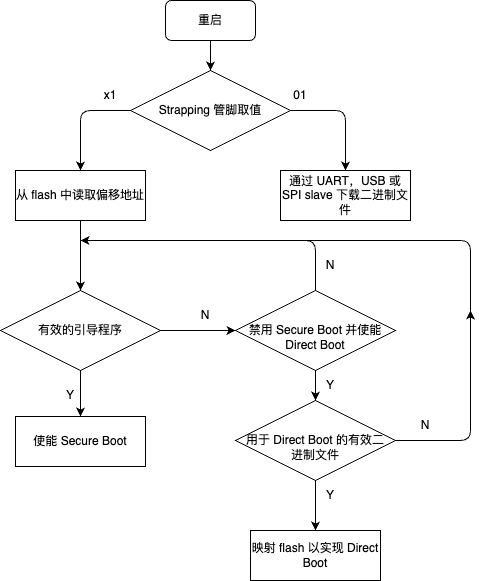
\includegraphics[scale=0.8]{13-BOOTCTRL/figures/chip_boot_flow_cn.png}}\\
    \textbf{注}：图中的 ``x1" 和 ``01" 为 Strapping 管脚 GPIO35 和 GPIO36 的组合值，见表 \ref{tab:bootctrl-boot-mode-control}。
    \caption{芯片 Boot 流程}
    \label{fig:boot_flow}
\end{figure}

下面几个 eFuse 比特位可用于控制 Boot 模式的具体行为：

\begin{itemize}
    \item \hyperref[fielddesc:EFUSEDISFORCEDOWNLOAD]{EFUSE\_DIS\_FORCE\_DOWNLOAD}

    如果此 eFuse 设置为 0（默认），软件可通过设置 \hyperref[fielddesc:LPSYSFORCEDOWNLOADBOOT]{LPSYSREG\_FORCE\_DOWNLOAD\_BOOT}，触发 CPU 复位，将芯片 Boot 模式强制从 SPI Boot 模式切换至 Joint Download 模式；如果此 eFuse 设置为 1，则禁用 \hyperref[fielddesc:LPSYSFORCEDOWNLOADBOOT]{LPSYSREG\_FORCE\_DOWNLOAD\_BOOT}。

    \item \hyperref[fielddesc:EFUSEDISDOWNLOADMODE]{EFUSE\_DIS\_DOWNLOAD\_MODE}

    如果此 eFuse 设置为 1，则禁用 Joint Download 模式。

    \item \hyperref[fielddesc:EFUSEENABLESECURITYDOWNLOAD]{EFUSE\_ENABLE\_SECURITY\_DOWNLOAD}

    如果此 eFuse 设置为 1，则在 Joint Download 模式下，只允许读取、写入和擦除明文 flash，不支持 L2MEM 或寄存器操作。如已禁用 Joint Download 模式，请忽略此 eFuse。

    \item \hyperref[fielddesc:EFUSEDISDIRECTBOOT]{EFUSE\_DIS\_DIRECT\_BOOT}

    如果此 eFuse 设置为 1，SPI Boot 模式下的 Direct Boot 会被禁用。
\end{itemize}

USB Serial/JTAG 控制器可将芯片从 SPI Boot 模式强制切换到 Joint Download 模式，或从 Joint Download 模式强制切换到 SPI Boot 模式。更多信息，请参考章节 \ref{mod:usbserialjtag} \textit{\nameref{mod:usbserialjtag}}。

可以设置 eFuse 位 \hyperref[fielddesc:EFUSEDISUSBSERIALJTAGDOWNLOADMODE]{EFUSE\_DIS\_USB\_SERIAL\_JTAG\_DOWNLOAD\_MODE} 来禁止 USB 串口/JTAG 控制器强制切换到 Joint Download 模式。

\subsection{ROM 代码日志打印控制}

系统在 SPI Boot 模式下的早期阶段，ROM 代码日志可打印至：

\begin{itemize}
    \item \textbf{（默认）UART0 和 USB 串口/JTAG 控制器}
    \item \textbf{UART0}
    \item \textbf{USB 串口/JTAG 控制器}
\end{itemize}

\hyperref[fielddesc:EFUSEUARTPRINTCONTROL]{EFUSE\_UART\_PRINT\_CONTROL} 和 GPIO36 控制 ROM 日志打印至 \textbf{UART0}，如表 \ref{tab:bootctrl-rom-code-printing-control} \nameref{tab:bootctrl-rom-code-printing-control} 所示。

\begin{table}[H]
    \centering
    \caption{ROM 日志打印}
    \label{tab:bootctrl-rom-code-printing-control}
    \begin{threeparttable}
    \begin{tabular}{ |p{1.3cm}<{\centering}|p{1.3cm}<{\centering}|p{4cm}|}
    \hline
        \rowcolor{lightgray}
    \textbf{eFuse\tnote{1}} &   \textbf{GPIO36}      & \textbf{ROM 代码日志打印} \\\hline
    0 &  x\tnote{2}  & 始终使能\\\hline
    \multirow{2}*{1}   & 0     & 使能 \\\cline{2-3}
     & 1       & 关闭 \\\hline
    \multirow{2}*{2}   & 0     & 关闭 \\\cline{2-3}
     & 1       & 使能 \\\hline
     3 &  x  & 始终关闭\\\hline
        \end{tabular}

        \begin{tablenotes}
            \item[1] eFuse: \hyperref[fielddesc:EFUSEUARTPRINTCONTROL]{EFUSE\_UART\_PRINT\_CONTROL}
            \item[2] x：任何取值均不会对结果有影响，因此可忽略。
        \end{tablenotes}
     \end{threeparttable}
    \end{table}

\hyperref[fielddesc:EFUSEDISUSBSERIALJTAGROMPRINT]{EFUSE\_DIS\_USB\_SERIAL\_JTAG\_ROM\_PRINT} 控制打印至 \textbf{USB 串口/JTAG 控制器}。该位为 1 时禁用打印至 USB 串口/JTAG 控制器。该位为 0，且 USB 串口/JTAG 控制器已通过 \hyperref[fielddesc:EFUSEDISUSBSERIALJTAG]{EFUSE\_DIS\_USB\_SERIAL\_JTAG} 开启，ROM 日志可打印到 USB 串口/JTAG 控制器。

注意，在 \hyperref[fielddesc:EFUSEDISUSBSERIALJTAGROMPRINT]{EFUSE\_DIS\_USB\_SERIAL\_JTAG\_ROM\_PRINT} 设置为 0，即可打印至 USB 的情况下，如果 USB 串口/JTAG 控制器已被禁用，则 ROM 代码将无法打印到 USB 串口/JTAG 控制器。

\subsection{JTAG 信号源控制}

在系统 Boot 早期阶段，GPIO34 与 \hyperref[fielddesc:EFUSEDISPADJTAG]{EFUSE\_DIS\_PAD\_JTAG}、\hyperref[fielddesc:EFUSEDISUSBJTAG]{EFUSE\_DIS\_USB\_JTAG} 和 \hyperref[fielddesc:EFUSEJTAGSELENABLE]{EFUSE\_JTAG\_SEL\_ENABLE} 一起控制 JTAG 信号源，见表 \ref{tab:bootctrl-jtag-signal-src-control}。

\begin{table}[H]
    \centering
    \caption{JTAG 信号源控制}
    \label{tab:bootctrl-jtag-signal-src-control}
    \begin{threeparttable}
    \begin{tabular}{ |p{1.3cm}<{\centering}|p{1.3cm}<{\centering}|p{1.3cm}<{\centering}|p{1.3cm}<{\centering}|p{8.5cm}| }
    \hline
        \rowcolor{lightgray}
        \textbf{eFuse 1\tnote{a}} & \textbf{eFuse 2\tnote{b}} & \textbf{eFuse 3\tnote{c}} &   \textbf{GPIO34}      & \textbf{JTAG 信号源} \\\hline
    \multirow{3}*{0} & \multirow{3}*{0} & 0 &  x\tnote{d}  & JTAG 信号来自 USB Serial/JTAG 控制器\\\cline{3-5}
    & & \multirow{2}*{1}   & 0     & JTAG 信号来自相应管脚 MTDI、MTCK、MTMS 和 MTDO\\\cline{4-5}
    & & & 1       & JTAG 信号来自 USB Serial/JTAG 控制器 \\\hline
    0 & 1 & x & x & JTAG 信号来自相应管脚 MTDI、MTCK、MTMS 和 MTDO\\\hline
    1 & 0 & x & x & JTAG 信号来自 USB Serial/JTAG 控制器\\\hline
    1 & 1 & x & x & JTAG 被禁用\\\hline
        \end{tabular}

        \begin{tablenotes}
            \item[a] eFuse 1: \hyperref[fielddesc:EFUSEDISPADJTAG]{EFUSE\_DIS\_PAD\_JTAG}
            \item[b] eFuse 2: \hyperref[fielddesc:EFUSEDISUSBJTAG]{EFUSE\_DIS\_USB\_JTAG}
            \item[c] eFuse 3: \hyperref[fielddesc:EFUSEJTAGSELENABLE]{EFUSE\_JTAG\_SEL\_ENABLE}
            \item[d] x：任何取值均不会对结果有影响，因此可忽略。
        \end{tablenotes}
     \end{threeparttable}
    \end{table}

\end{document}
